\documentclass[titlepage]{article}
\usepackage{amsmath}
\usepackage{amsfonts}
\usepackage[T1]{fontenc}
\usepackage{tikz}
\usepackage{tikz-qtree}
\usepackage{forest}
\usepackage[style=numeric]{biblatex}
\usepackage{amsthm}
\usepackage{mathtools}
\usepackage{stmaryrd}
\usepackage{algorithm}
\usepackage{algpseudocode}
\usepackage{tabularx,ragged2e,booktabs,caption}
\usepackage{graphicx}



\addbibresource{refs.bib}
%\newtheoremstyle{break}{10pt}{0pt}{}{}{\bfseries}{}{\newline}{}
%\theoremstyle{break}
\newtheorem{theorem}{Theorem}
\newtheorem{lemma}{Lemma}
\newtheorem{definition}{Definition}
\newtheorem{example}{Example}
\newtheorem{proposition}{Porposition}

\newcommand*{\textcal}[1]{%
  % family qzc: Font TeX Gyre Chorus (package tgchorus)
  % family pzc: Font Zapf Chancery (package chancery)
  \textit{\fontfamily{qzc}\selectfont#1}%
}

%\newcommand{\Tmc}{\ensuremath{\mathcal{T}}\xspace}
\DeclareMathOperator{\st}{st}

\begin{document}
\section{Introduction}
Description Logics (DLs) are a family of formal logics designed for representing and inferring new
knowledge from defined knowledge encapsulated in ontologies. However, some ontologies like SNOMED or
LOINC \cite{article}
contain a vast number of axioms, making it challenging to extend them without generating unwanted 
inferences. Proofs, which are essentially trees consisting of axioms as vertices connected by 
direct consequence operators, can be useful in understanding the cause of these unwanted inferences. 
Recently, a new Java library called Evee-libs \cite{https://doi.org/10.48550/arxiv.2206.07711} has been developed to generate proofs for DLs up to 
$\mathcal{ALCH}$. To achieve this, Evee-libs uses Lethe \cite{KoopmannSchmidt15c}, a 
consequence-based reasoning procedure, to generate new axioms. However, the underlying direct 
consequence operator, which is Lethes underlying calculus, 
plays a critical role in determining the resulting proofs. Therefore, in this student project report, 
I will present an implementation of the alternative calculus proposed in [3] and compare the 
generated proofs to those of Evee-libs. This comparison will provide valuable insights into the effectiveness of 
different calculi in generating proofs for ontologies, which could ultimately lead to improved 
methods for extending and reasoning about ontologies.



\section{The Description Logic $\mathcal{ALCH}$}

\subsection{Syntax}
The DL $\mathcal{ALCH}$ allows the operators concept negation ($\neg$), 
concept intersection ($\sqcap$), concept union ($\sqcup$), value restriction
 ($\forall$), existential restriction ($\exists$), the top concept ($\top$),
 the bottom concept ($\bot$) and finally general concept inclusions (GCIs) ($\sqsubseteq$).
With those operators and two additional sets of concept names ($N_C$) and role names ($N_R$),
one can then build all complex concepts of $\mathcal{ALCH}$ 
($C_{\mathcal{ALCH}}$) as follows:

    \begin{tabular}{l l}
      if $C \in N_C$ & then $C \in N_{\mathcal{ALCH}}$ \\
      if $C \in N_{\mathcal{ALCH}}$ & then $\neg C \in N_{\mathcal{ALCH}}$ \\
      if $C_1,C_2 \in N_{\mathcal{ALCH}}$ & then $C_1 \sqcap C_2 \in N_{\mathcal{ALCH}}$ \\
      if $C_1,C_2 \in N_{\mathcal{ALCH}}$ & then $C_1 \sqcup C_2 \in N_{\mathcal{ALCH}}$ \\
      if $C \in N_{\mathcal{ALCH}}$ and $r \in N_R$ & then $\exists r.C \in N_{\mathcal{ALCH}}$ \\
      if $C \in N_{\mathcal{ALCH}}$ and $r \in N_R$ & then $\forall r.C \in N_{\mathcal{ALCH}}$ \\
    \end{tabular} 
    %TODO: different place?
    Note that concept names and negated concept names are called literals
    
    

Now that complex concepts are defined we can also formalize the notion of a TBox.
\begin{definition}[TBox]
  An $\mathcal{ALCH}$ TBox $\mathcal{T}$ is a finite set of general concept inclusions and role inclusions
   i.e. $\mathcal{T} \subseteq \{C_1 \sqsubseteq C_2 \mid C_1, C_2 \in N_{\mathcal{ALCH}} \} \cup 
  \{r_1 \sqsubseteq r_2 \mid r_1, r_2 \in N_R\}$
\end{definition}

%TODO: ask if ABox is needed
\begin{definition}[ABox]
  An ABox $\mathcal{A}$ is a finite set of concept and role assertions i.e.
  $\mathcal{A} \subseteq \{a:C \mid a \in N_I, C \in N_{\mathcal{ALCH}}\}
  \cup \{(a,b):r \mid a,b \in N_I, r \in N_R\}$
\end{definition}

\begin{definition}[Ontology]
  An Ontology $\mathcal{O}$ is a pair $(\mathcal{T}, \mathcal{A})$ of a TBox $\mathcal{T}$ and an ABox $\mathcal{A}$
\end{definition}

%TODO correct place?
In order to later define a normal form for an ontology, we need to define the notion of a concept
to occur positively or negatively in an ontology.
\begin{definition}
  Let $\mathcal{O} = (\mathcal{T}, \mathcal{A})$ some ontology and $C$ some concept then we say that a concept $C$ occurs positively (negatively) in $\mathcal{O}$ if
  $C$ occurs positively (negatively) in some GCI of $\mathcal{T}$. \\
  \begin{itemize}
    \item $C$ occurs positively in itself.
    \item If $C$ occurs positively (negatively) in C' then C occurs positively (negatively) in
    $C' \sqcap D C \sqcap D', C' \sqcup D, C \sqcup D', \exists r.C', \forall r.C'$ 
    and negatively (positively) in $\neg C'$.
  \end{itemize}
  



  
\end{definition}


\subsection{Semantics}
The semantics of the DL $\mathcal{ALCH}$ are defined by a first order logic interpretation
$I := (\Delta^I, \cdot^I)$, where $\Delta^I$ is the \emph{domain} of the interpretation
and $\cdot^I$ the interpretation function which assigns to:
\begin{itemize}
  %I do not need individual names right? 
  %\item every individual name $a \in N_I$ a member $a^I \in \Delta^I$
  \item every concept name $A \in N_C$ a subset $A^I \subseteq \Delta^I$
  \item every role name $r \in N_R$ a binary relation $r^I \subseteq \Delta^I \times \Delta^I$
\end{itemize}
First 
Concepts are then interpreted as follows:
\begin{definition}[Interpretation]
  Let $A \in N_C, C, D \in N_{\mathcal{ALCH}}, r \in N_R$ then
  \begin{center}
    \begin{tabular}{l c l}
      %use align* * := ohne nummerierung
    
      $\top^I$& $\coloneqq$& $\Delta^I$ \\
      $\bot^I$& $\coloneqq$& $\emptyset$\\      
      %$A^I$ & $\coloneqq$ & $A'$ where $A' \subseteq \Delta^I$ \\
      %$r^I$ & $\coloneqq$ & $R$ where $R \subseteq \Delta^I \times \Delta^I$\\
      $(\neg C)^I$ & $\coloneqq$ & $C^I$ \\
      $(C \sqcap D)^I$ & $\coloneqq$ & $C^I \cap D^I$ \\
      $(C \sqcup D)^I$ & $\coloneqq$ & $C^I \cup D^I$ \\
      $(\exists r.C)^I$ & $\coloneqq$ & $ \{a \in \Delta^I \mid \exists b \in \Delta^I : (a,b) \in r^I \text{ and } b \in C^I \}$ \\
      $(\forall r.C)^I$ & $\coloneqq$ & $ \{a \in \Delta^I \mid \forall b \in \Delta^I : \text{if} (a,b) \in r^I \text{, then } b \in C^I \}$ \\
      \end{tabular}        
  \end{center}
\end{definition}

GCIs and role inclusions are used to express constrains which have to
be satisfied by an interpretation. To express that an interpretation satisfies a GCI
or a role inclusion the satisfaction operator ($\models$) is used. 

\begin{definition}
    For $C, D \in N_{\mathcal{ALCH}}: I \models C \sqsubseteq D  :\iff C^I \subseteq D^I$ \\
    For $r, s \in N_R: I \models r \sqsubseteq s  :\iff r^I \subseteq s^I$
\end{definition}


%TODO: ask if this is needed
This definition can be extended to TBoxes and Ontologies. Usually also the ABox
has to be satisfied by an interpretation, but since the algorithm only reasons over the TBox,
 I will not define it here.
\begin{definition}
  For $\mathcal{T} TBox $
  $I \models \mathcal{T} :\iff I \models C \sqsubseteq D \text{ for all } C \sqsubseteq D \in \mathcal{T}$ \\
  $I \models \mathcal{O} :\iff I \models \mathcal{T} \text{ and } I \models \mathcal{A}$
\end{definition}

Another very important concept is that ontologies can entail some GCI or role inclusion.
This is particular important since we want to find proofs for such entailments.
% TODO: entailment or derivation?
\begin{definition}
  Let $\mathcal{O}$ ontology, $C \sqsubseteq D$ GCI and $r \sqsubseteq s$ role inclusion.
  Then 
  \begin{itemize}
    \item $\mathcal{O} \models C \sqsubseteq D$ iff for all interpretations $I$
    if $I \models \mathcal{O}$ then $I \models C \sqsubseteq D$
    \item $\mathcal{O} \models r \sqsubseteq s$ iff for all interpretations $I$
    if $I \models \mathcal{O}$ then $I \models r \sqsubseteq s$
  \end{itemize} 

\end{definition}






\section{The Algorithm}
In this section I will describe how my algorithm works and therefore start with what a
proof formally is.

\subsection{Proofs}
Proofs capture the logical derivation structure of an GCI, which is entailed by some Ontology and 
therefor we define a proof for some $\mathcal{O} \models \alpha $ as defined in \cite{10.1007/978-3-031-10769-6_16} 
as finite, acyclic, directed, labeled hypergraphs G = (V, E, l) where V is a finite set of vertices, 
E is a finite set of hyperedges $(S,d)$, where $S \subseteq V$ and $d \in V$
and $l$ a labeling function that assigns GCIs to vertices. Note that leaves must be labeled by Ontology GCIs and
$\alpha$ has to be the label for the root vertex. Hyperedges are also restricted further such that  
$\{l(v) \mid v \in S \} \models l(d)$ has to hold.

%A proof is a list of GCIs $A_1, \ldots, A_n$, where for each $i \in \{1, \ldots n - 1\}
%$ $\{A_1, \ldots, A_i\} \models A_{i+1}$. Since my approach uses rules to derive such
%proofs I now define a rule based definition of a proof. A rule based proof is not a list
%of GCIs but rather a list of inferences, where an inference is a tuple $((\phi_1, \ldots, \phi_n), \psi, \mathbf{R})$,
%where $\phi_1, \ldots, \phi_n,$ are GCIs and the list containing them is called premise, $\psi$ is also a GCI
%and called the conclusion and $\mathbf{R}$ is a rule. In order a list of inferences
%to be a proof it has to hold that for all inferences the premise and conclusion actually have to be an 
%instance of $\mathbf{R}$.


\subsection{Normalization}\label{alg:norm}
Before we dive into the rule based procedure, we first need to be sure, that our ontology has the right form.
\begin{definition}[Normal form]
  An ontology $\mathcal{O}$ is said to be in normal form, iff all axioms in $\mathcal{O}$ are of the form
  $\bigsqcap A_i \sqsubseteq \bigsqcup B_j, A \sqsubseteq \exists r.B, \exists r.A \sqsubseteq A, A \sqsubseteq \forall r.B$ 
  or $r \sqsubseteq s$, where $A_i, B_j, A, B $ are concept names and $r,s$ are role names. \cite{article}
\end{definition}
An $\mathcal{ALCH}$ ontology $\mathcal{O}$ can be easily transformed into this normal form by first 
removing all negative occurrences of the form $\forall r. C$ and replacing them with $\neg \exists r. \neg C$.
$\st(\mathcal{O})$ needs then to be further normalized by removing all concepts of the form $\forall r.C \sqsubseteq A$ and
replacing them with the logical equivalent concept $\neg \exists r. \neg C $.
Then we use the structural transformation operator $\st$ to transform the ontology into a new ontology $\st(\mathcal{O})$.
\emph{structural transformation} $\st: N_C \rightarrow N_C$. $\st$ is defined as follows:

\begin{center}

\begin{tabular}{l l }
$\st(A) \coloneqq  A$ & $\st(C \sqcap D) \coloneqq  [C] \sqcap [D]$\\
$\st(\top) \coloneqq \top$ & $\st(C \sqcup D) \coloneqq [C] \sqcup [D]$ \\
$\st(\bot) \coloneqq \top$ & $\st(\exists r.C) \coloneqq \exists r.[C]$\\
$\st(\neg C) \coloneqq \neg [C]$ & $\st(\exists r.C) \coloneqq \exists r.[C]$\\
\end{tabular}
\end{center}
where for a concept $C$ [C] is just a new atom that corresponds to $C$.
Now we obtain a new structurally transformed ontology $\st(\mathcal{O})$ form $\mathcal{O}$ by
first adding all role inclusions of $\mathcal{O}$ into it and then adding 
\begin{itemize}
  \item $\st(C) \sqsubseteq [C]$ for every negative $ C \in \mathcal{O}$ 
  \item $[D]\sqsubseteq \st(D)$ for every positive $D \in \mathcal{O}$
  \item $[C] \sqsubseteq [D]$ for every axiom $C \sqsubseteq D$ occuring $C \in \mathcal{O}$
\end{itemize}

Finally the following normalization rules have to be applied to $\st(\mathcal{O})$ until no rule can be applied
anymore.

  \begin{itemize}
    \item $ \dfrac{[C \sqcap D] \sqsubseteq [C] \sqcap [D]}{ [C \sqcap D] \sqsubseteq [C], \quad [C \sqcap D] \sqsubseteq [D]}$
    \item $ \dfrac{[C] \sqcup [D] \sqsubseteq [C \sqcup D]}{ [C] \sqsubseteq [C \sqcup D], \quad [D] \sqsubseteq [C \sqcup D]}$
    \item $ \dfrac{[\neg C] \sqsubseteq \neg [C] }{ [\neg C ] \sqcap [C] \sqsubseteq \bot}$
    \item $ \dfrac{\neg [C] \sqsubseteq [\neg C] }{ \top \sqsubseteq [\neg C ] \sqcap [C]}$
  \end{itemize}

\subsection{Inference rules}
\begin{definition}[Inference Rules]
  On a normalized ontology we can now apply the following inference rules.

\begin{align}
  \mathbf{R^{+}_A} & \dfrac{}{H\sqsubseteq A} : A \in H \label{rules:RPlusA}\\
  \mathbf{R^{-}_A} & \dfrac{H \sqsubseteq N \sqcup A}{H \sqsubseteq N} : \neg A \in H  \label{rules:RMinusA}\\ 
  \mathbf{R^{n}_{\sqcap}} & \dfrac{\{H \sqsubseteq N_i \sqcup A_i \}^{n}_{i=1}}{H \sqsubseteq \bigsqcup^{n}_{i=1} N_i \sqcup M} : \bigsqcap^{n}_{i=1} A_i \sqsubseteq M \in \mathcal{O} \label{rules:RNAnd} \\
  \mathbf{R^+_{\exists}} & \dfrac{H \sqsubseteq N \sqcup A }{ H \sqsubseteq N \sqcup \exists r.B} : A \sqsubseteq \exists r.B \in \mathcal{O} \label{rules:RPlusExists}\\
  \mathbf{R^-_{\exists}} & \dfrac{H \sqsubseteq M \sqcup \exists r.K,\quad K \sqsubseteq N \sqcup A}{H \sqsubseteq M \sqcup B \sqcup \exists r.(K \sqcap \neg A)} : \exists s.A \sqsubseteq B \in \mathcal{O} \quad r \sqsubseteq_{\mathcal{O}} s \label{rules:RMinusExists}\\
  \mathbf{R^\bot_{\exists}} & \dfrac{H \sqsubseteq M \sqcup \exists r.K,\quad K \sqsubseteq \bot}{H \sqsubseteq M} \label{rules:RBotExists}\\
  \mathbf{R_{\forall}} & \dfrac{H \sqsubseteq M \sqcup \exists r.K,\quad H \sqsubseteq N \sqcup A}{H \sqsubseteq M \sqcup N \sqcup \exists r.(K \sqcap B)} : A \sqsubseteq \forall s.B \in \mathcal{O} \quad r \sqsubseteq_{\mathcal{O}} s \label{rules:RForall}
\end{align}

where $M,N$ are disjunctions of concept names and $H,K$ are conjunctions of literals.
\end{definition}

%TODO: look up
\begin{algorithm}
  \caption{Main Loop}\label{alg:cap}
\begin{algorithmic}
  \Procedure{main}{ontology, goal}
  \State Normalizer.normalize(ontology)

  \State proofHandler $\gets$ new ProofHandler(qoal)
  \State rules $\gets$ getRules(ontology, proofHandler) 
  \While{notFinished(proofHandler)} 
  \For{(rule in rules)}
    \State setNewRule(rule.apply())
  \EndFor
  \EndWhile
  \EndProcedure
\end{algorithmic}
\end{algorithm}


The algorithm's main loop consists of two stages: normalization and rule application.
The normalization stage implements the algorithm as outlined in Section \ref{alg:norm}. The normalized
ontology and a new instance of a ProofHandler are then used to create instances of each rule type. 
Every rule, except for \ref{rules:RPlusA}, \ref{rules:RMinusA} and \ref{rules:RBotExists}   which do not need ontology axioms, need these two as 
arguments. The ontology is preprocessed, such that all relevant ontology axioms are saved in a way which 
allows for an easier rule application and prevents searching for relevant axioms every time the rule is 
applied. The ProofHandler provides active axioms from which rules are able to create new axioms and processes
them, as described in Section \ref{alg:proofHandler}, to generate new inferences. The created rules are then applied 
one after the other until the halting condition is met.  The halting condition is set to true either when 
the goal concept is reached or when all rules are unable to generate a new axiom in an iteration. 


%TODO how to call C, D in C subseteq D ? 
\subsection{Proof Handler}\label{alg:proofHandler}
The ProofHandler is the main component of the algorithm. It is responsible for handling new produced axioms,
provides the rules with these new axioms, checks whether the halting condition is met and creates a proof
in case the algorithm finds one. The ProofHandler is initialized with the goal axiom. The subconcept of this
axiom is added to the list of active axioms and the super concept is saved in order to check whether the goal
was found. The handling of newly produced axioms contains the following steps. First the ProofHandler is provided
with all axioms which were used to generate, the new axiom the newly generated axiom and the name of the rule which 
calls the method. In case of rules which also use ontology axioms
the provided axioms are split into premises and ontology premises. This information is then used to create a new
Inference and add the new axiom to the list of active Axioms. Since some rules do generate some axioms multiple
times the ProofHandler also checks whether the axiom is already in the list of active axioms and depending on
the outcome of this check returns the information whether a new Inference was created. While doing so it is also
checked whether the super concept of the new axiom is the goal axiom. In case the algorithm stops
and the goal was found the ProofHandler also provides a method to create a proof. In order to prevent to just
return all Inferences which were created during the algorithm the ProofHandler uses the Java library EVEE to extract
a meaningful proof.
EVEE not only provides data structures like Inferences and Proofs but also has different algorithms to create
different types of proofs. In this project I use the algorithm which extracts a proof with the lowest depth possible.


\subsection{Inference Rules}\label{alg:rules}
In this subsection, I will describe how each inference rule is implemented and what data structures they use.
%ITS IMPORTANT TO FLATTEN CONCEPTS
% and empty conjunctions and conjunctions with only one element !!!!!

%In this subsection I will describe how the inference rules are implemented. Let's start
%which inputs and output types of each rule implementation. Most rule implementations
% need two kinds of resources. Axioms which are part of the given ontology and axioms, which are
%active. An axiom is said to be active if it was previously created by some rule. This is 
%not the case for rule \ref{rules:RPlusA}, \ref{rules:RMinusA} and \ref{rules:RBotExists}. Instead, the rules \ref{rules:RPlusA} and \ref{rules:RMinusA} use active concepts to
%produce new axioms, where active concepts, similar to active axioms, are concepts, which
%were created by some rule. The rule (1) does not even use any active axioms. And all rules
%have in common, that they produce on each application, but it is not so simple for the 
%rule implementations. Due to the matching process most rules produce in one application
%more than one axiom. Now I will go over every rule in more detail and will describe of 
%they were implemented
\subsubsection{The rule $\mathbf{R^{+}_A} \coloneq \dfrac{}{H\sqsubseteq A} : A \in H \label{rules:RPlusA}\\$}
The rule \ref{rules:RPlusA} is one of the simplest rules, since it does not use any active axioms and
also no axioms from the ontology. The only thing that has to be taken care of is
creating new axioms from active concepts. In order to do that, the implementation iterates
through all active concepts and searches for conjunctions or concept names, which are seen as conjunctions of size 1.
In case a conjunction $H$ is found, all concept names $A$ within the conjunction are saved to a list.
Each element $A$ is then used as superconcept of a new axiom with its origin $H$ as subconcept.
After the handling of all active concepts, the implementation empties the list of active concepts in order to
reduce redundant axiom creation.

\subsubsection{The rule $\mathbf{R^{-}_A} \coloneq \dfrac{H \sqsubseteq N \sqcup A}{H \sqsubseteq N} : \neg A \in H  \label{rules:RMinusA}$}
This rule also does not use any axioms from the ontology but does use active axioms.
The implementation first searches for axioms with a conjunction $H$ as subconcept, that contains negative
literals. In case such an axiom $H$ was found the implementation searches for each negative literal $\neg A$ in $H$ for
 the positive literal $A$ in the superconcept
$N \sqcup A$ of the axiom. 
If the superconcept contains the positive literal the implementation creates a new axiom with 
the same sub concept as the origin axiom and the superconcept of the origin axiom without the positive literal.
Note that used active axioms are not removed from the list of active axioms, which allows the possibility of
redundant axiom creation. In order to tackle this problem I created an alternative rule implementation
which checks before handling an active axiom
whether it was already used by this rule. To achieve this, the rule stores all used axioms in a set. This set can 
become very large and in worst case can contain all active axioms. That's why I made it an alternative implementation
in order to allow for a time-optimized version of the algorithm and a space-optimized version of the algorithm.

\subsubsection{The rule $\mathbf{R^{n}_{\sqcap}} \coloneq \dfrac{\{H \sqsubseteq N_i \sqcup A_i \}^{n}_{i=1}}{H \sqsubseteq \bigsqcup^{n}_{i=1} N_i \sqcup M} : \bigsqcap^{n}_{i=1} A_i \sqsubseteq M \in \mathcal{O} \label{rules:RNAnd}$}
The rule \ref{rules:RNAnd} is the first rule which uses axioms from the ontology.
On initialization of the rule first the ontology, which is passed to it, 
gets filtered for axioms of the form $\bigsqcap^{n}_{i=1} A_i \sqsubseteq M$
These axioms get saved into a list of tuples where the first element of the tuple is the conjunction
$\bigsqcap^{n}_{i=1} A_i$
stored as a set $\{A_1 \ldots A_n\}$ and the second element is the entire axiom $\bigsqcap^{n}_{i=1} A_i \sqsubseteq M$, 
which will not only be used to get its superconcept
for creation of a new axiom, but also in order to pass it as ontology premise to the ProofHandler.
On application of the rule the following 
function $m  \coloneqq N_{\mathcal{ALCH}} \times N_C \rightarrow \text{list}(\{N \mid N \subseteq N_C\})$
is defined by using the current active axioms. First all active axioms get filtered for
axioms of the form $H \sqsubseteq N \sqcup A$, where $H$ is a conjunction of literals, $N$ a disjunction
 of concept names and $A$ an atom. Every axiom is then used to define the function m in the following way:
 For each active axiom $\alpha = H \sqsubseteq N \sqcup A: m(H,A) \coloneqq \langle \{N_c \mid N_c \in N\} \mid \rangle$.
 Note that there can be multiple active axioms with the same subconcept $H$ and the same atom $A$ but with different 
 $N_1$ and $N_2$ and therefore m maps to a list of sets.
 After the function is defined it will be used to compose derived axioms.
 In order to do so the implementation first iterates through all ontology axioms and checks
 whether the LHS of a given axiom is subsumed by $A$. If this is
 the case, m can be used to find for all $A_i$ in the matched ontology axiom the corresponding
 $N_i$ and in the end the new axiom $H \sqsubseteq \bigsqcup^{n}_{i=1} N_i \sqcup M$ is created.
 Note that due to m mapping to a list multiple axioms can be created. 



%When the rule is applied to the set of active axioms the rule first maps all axioms
%with an equal subconcept to a tuple, where the first entry is a list of concept names,
%which where these concept names corresponds to all $A_i$ which can be found for a given
%subconcept $H$ and the second entry is a map which maps a concept name which 
%is a particular $A_i$ and maps it to a tuple where its first entry is a list of all concept 
%names in the corresponding $N_i$ and the second entry is just the hole axiom 
%$H \sqsubseteq N_i \sqcup A_i$. 

%After the map is created the rule starts to iterate 
%through the ontology axioms and the created entries of the just created map and looks for
%entries in the map where the set of $A_i$s from the list, which was created from the ontology,
%is subsumed by some set in the set in first entry of the map.
%When such a match was found we have all need elements to create the new axiom 
%$H \sqsubseteq \bigsqcup^{n}_{i=1} N_i \sqcup M$ in order to get all required $N_i$s
%the list of $A_i$s of the ontology axiom is used to filter the map in the second entry
%of the entry of the just created map.

\subsubsection{The rule $\mathbf{R^+_{\exists}} \coloneq \dfrac{H \sqsubseteq N \sqcup A }{ H \sqsubseteq N \sqcup \exists r.B} : A \sqsubseteq \exists r.B \in \mathcal{O}$}
The rule (4) also uses axioms from the ontology so on creation of the rule
 implementation the ontology gets filtered for axioms of the form 
 $A \sqsubseteq \exists r.B \in \mathcal{O}$. When the rule implementation is applied,
 it matches to every applicable ontology axioms all active axioms for axioms of the form
  $H \sqsubseteq N \sqcup A$ and creates a new axiom $H \sqsubseteq N \sqcup \exists r.B$ in case
  such a match is found.


 %\subsubsection{The rule $\mathbf{R^-_{\exists}} \coloneq \dfrac{H \sqsubseteq M \sqcup \exists r.K,\quad K \sqsubseteq N \sqcup A}{H \sqsubseteq M \sqcup B \sqcup \exists r.(K \sqcap \neg A)} : \exists s.A \sqsubseteq B \in \mathcal{O} \quad r \sqsubseteq_{\mathcal{O}} s$}
 \subsubsection{
  \begin{tabular}{ll}
    $\mathbf{R^-_{\exists}} \coloneq $&$\dfrac{H \sqsubseteq M \sqcup \exists r.K,\quad K \sqsubseteq N \sqcup A}{H \sqsubseteq M \sqcup B \sqcup \exists r.(K \sqcap \neg A)} :$\\
    &$A \sqsubseteq \forall s.B \in \mathcal{O} \quad r \sqsubseteq_{\mathcal{O}} s$
\end{tabular}
 }
 
 The rule (5) not only uses axioms from the ontology but also uses role inclusions that
follow from the ontology. The role inclusions are calculated separately since rule (7) 
also uses them. So the only thing that has to be done on creation is, that axioms of the form
$\exists s.A \sqsubseteq B$ need to be filtered and afterwards fitting role inclusions ares searched for
and safed together in a list. 
On rule application the rule implementation then iterates through all found ontology axioms and role inclusions
and searches for active axioms of the form  $K \sqsubseteq N \sqcup A$. If such an axiom is found
one then searches for active axioms of the form $H \sqsubseteq M \sqcup \exists r.K$. by using the
just found subconcept $K$. If such an axiom is found the new axiom $H \sqsubseteq M \sqcup B \sqcup \exists r.(K \sqcap \neg A)$
is created.


\subsubsection{The rule $\mathbf{R^\bot_{\exists}} \coloneq \dfrac{H \sqsubseteq M \sqcup \exists r.K,\quad K \sqsubseteq \bot}{H \sqsubseteq M}$}
The rule (6) does not use axioms from the original ontology. Usually there are way more axioms that contain existential restrictions 
in ontologies, which I used for testing,
than axioms with the bottom concept on the right-hand side, and
therefore the implementation first filters for axioms of the form $K \sqsubseteq \bot$ safes them
in a list $l$. Afterwards
the rule implementation filters for rules of the form $H \sqsubseteq M \sqcup \exists r.K $
and checks if an axiom of this form is found, if the K already occures in some LHS of an axiom in
$l$. From this found rule then the new axiom $H \sqsubseteq M$ can then be created immediately.

\subsubsection{The rule $\mathbf{R_{\forall}}$}
The rule (7) is no the final rule now again uses from the ontology following role inclusions
and also axioms from the ontology of the form $A \sqsubseteq \forall s.B$. Therefore, on 
creation of the rule implementation first the ontology gets filtered for such axioms, where 
the role s is on the right-hand side of some implied role inclusion.
On application of the rule implementation first searches for active axioms of the form
$H \sqsubseteq M \sqcup \exists r.K$ where r has to match some RHS of some matched role inclusion.
The found axioms are then used to define a function $m_l \coloneqq N_ \rightarrow$


\begin{example}
  Let $\mathcal{O} = \{ B \sqsubseteq \exists r.D, A \sqsubseteq \forall s.E, \exists r.E \sqsubseteq C, r \sqsubseteq s\}$
  then a proof for $A \sqcap B \sqsubseteq C $ would look like the following: \\
    $(((),A \sqcap B \sqsubseteq B, \mathbf{R^+_A}),$ \\
    $((A \sqcap B \sqsubseteq B, B \sqsubseteq \exists r.D), A \sqcap B \sqsubseteq \exists r.D, \mathbf{R^+_{\exists}}), $ \\
    $((A \sqcap B \sqsubseteq \exists r.D, A \sqsubseteq \forall s.E, r \sqsubseteq s),A \sqcap B \sqsubseteq \exists r.(D \sqcap E), \mathbf{R_{\forall}}), $ \\
    $((),(D \sqcap E) \sqsubseteq E, \mathbf{R^+_A}),$ \\
    $((A \sqcap B \sqsubseteq \exists r.(D \sqcap E), (D \sqcap E) \sqsubseteq E, \exists r.E \sqsubseteq C), A \sqcap B \sqsubseteq \exists r.(D \sqcap E \sqcap \neg E) \sqcup C, \mathbf{R^-_{\exists}}),$ \\
    $((), D \sqcap E \sqcap \neg E \sqsubseteq E, \mathbf{R^+_A}), $ \\
    $((D \sqcap E \sqcap \neg E \sqsubseteq E),D \sqcap E \sqcap \neg E \sqsubseteq \bot, \mathbf{R^-_A}),$ \\
    $((A \sqcap B \sqsubseteq \exists r.(D \sqcap E \sqcap \neg E) \sqcup C, D \sqcap E \sqcap \neg E \sqsubseteq \bot), A \sqcap B \sqsubseteq C, \mathbf{R^{\bot}_{\exists}}))$
\end{example}
Notes that in the algorithm not only these concepts would be created but also other rules.
For example even in the first step not only $A \sqcap B \sqsubseteq B$ would have been created but also
$A \sqcap B \sqsubseteq A$.



\section{Results}



\begin{table}[h]
  \centering
  \begin{tabular}{|c|c|c|c|c|}
    \hline
    \textbf{Task} & \textbf{Time (ms)} & \textbf{\#Axioms} & \textbf{Size largest Premise} & \textbf{\#RuleApplications} \\
    \hline
    00001 & 192 & 19 & 3 & 20  \\
    00003 & 5913 & 23 & 4 & 27 \\
    00008 & 133 & 15 & 3 & 18  \\
    00009 & 119 & 25 & 4 & 27  \\
    00012 & 24 & 7 & 2 & 7  \\
    \hline
  \end{tabular}
  \caption{Performance of the ALCH-Reasoner}
  \label{tab:alch-performance} 
\end{table}



\begin{table}[h]
  \centering
  \begin{tabular}{|c|c|c|c|c|}
    \hline
    \textbf{Task} & \textbf{Time (ms)} & \textbf{\#Axioms} & \textbf{Size largest Premise} & \textbf{\#RuleApplications} \\
    \hline
    \hline
    00001 & 2786 & 13 & 2 & 13 \\
    00003 & 502 & 5 & 2 & 5  \\
    00008 & 2728 & 8 & 2 & 8  \\
    00009 & 1348 & 11 & 2 & 11 \\
    00012 & 159 & 2 & 1 & 2  \\
    \hline
  \end{tabular}
  \caption{Performance of the Lethe}
    \label{tab:lethe-performance}
\end{table}

  
    
  
\subsection{Setup}
In order to compare the performance of the ALCH-Reasoner in terms of time consumption and also
readability of the proofs, I used Lethe \cite{KoopmannSchmidt15c}, as a reference.
Lethe is integrated into EVEE and I use the LetheBasedALCHProofGenerator to access it.
Lethe is a uniform interpolation (UI) tool which uses a resolution based calculus to compute
proofs for different DLs up to $\mathcal{ALCH}$.

The dataset I use to compare the two approaches is a dataset created in \cite{DBLP:conf/cade/AlrabbaaBBDKM22}
It basically consists of justifications for axioms in the Bioportal-Repository, which where renamed,
resulting in so-called justification patterns. Some of these patterns are quite challenging to 
compute proofs for, which is why I chose only a small subset of the dataset. Also, some of the tasks
use domain specifications which I do not support.



\subsection{Proofs Shape Comparison}
\begin{figure}
  \centering
  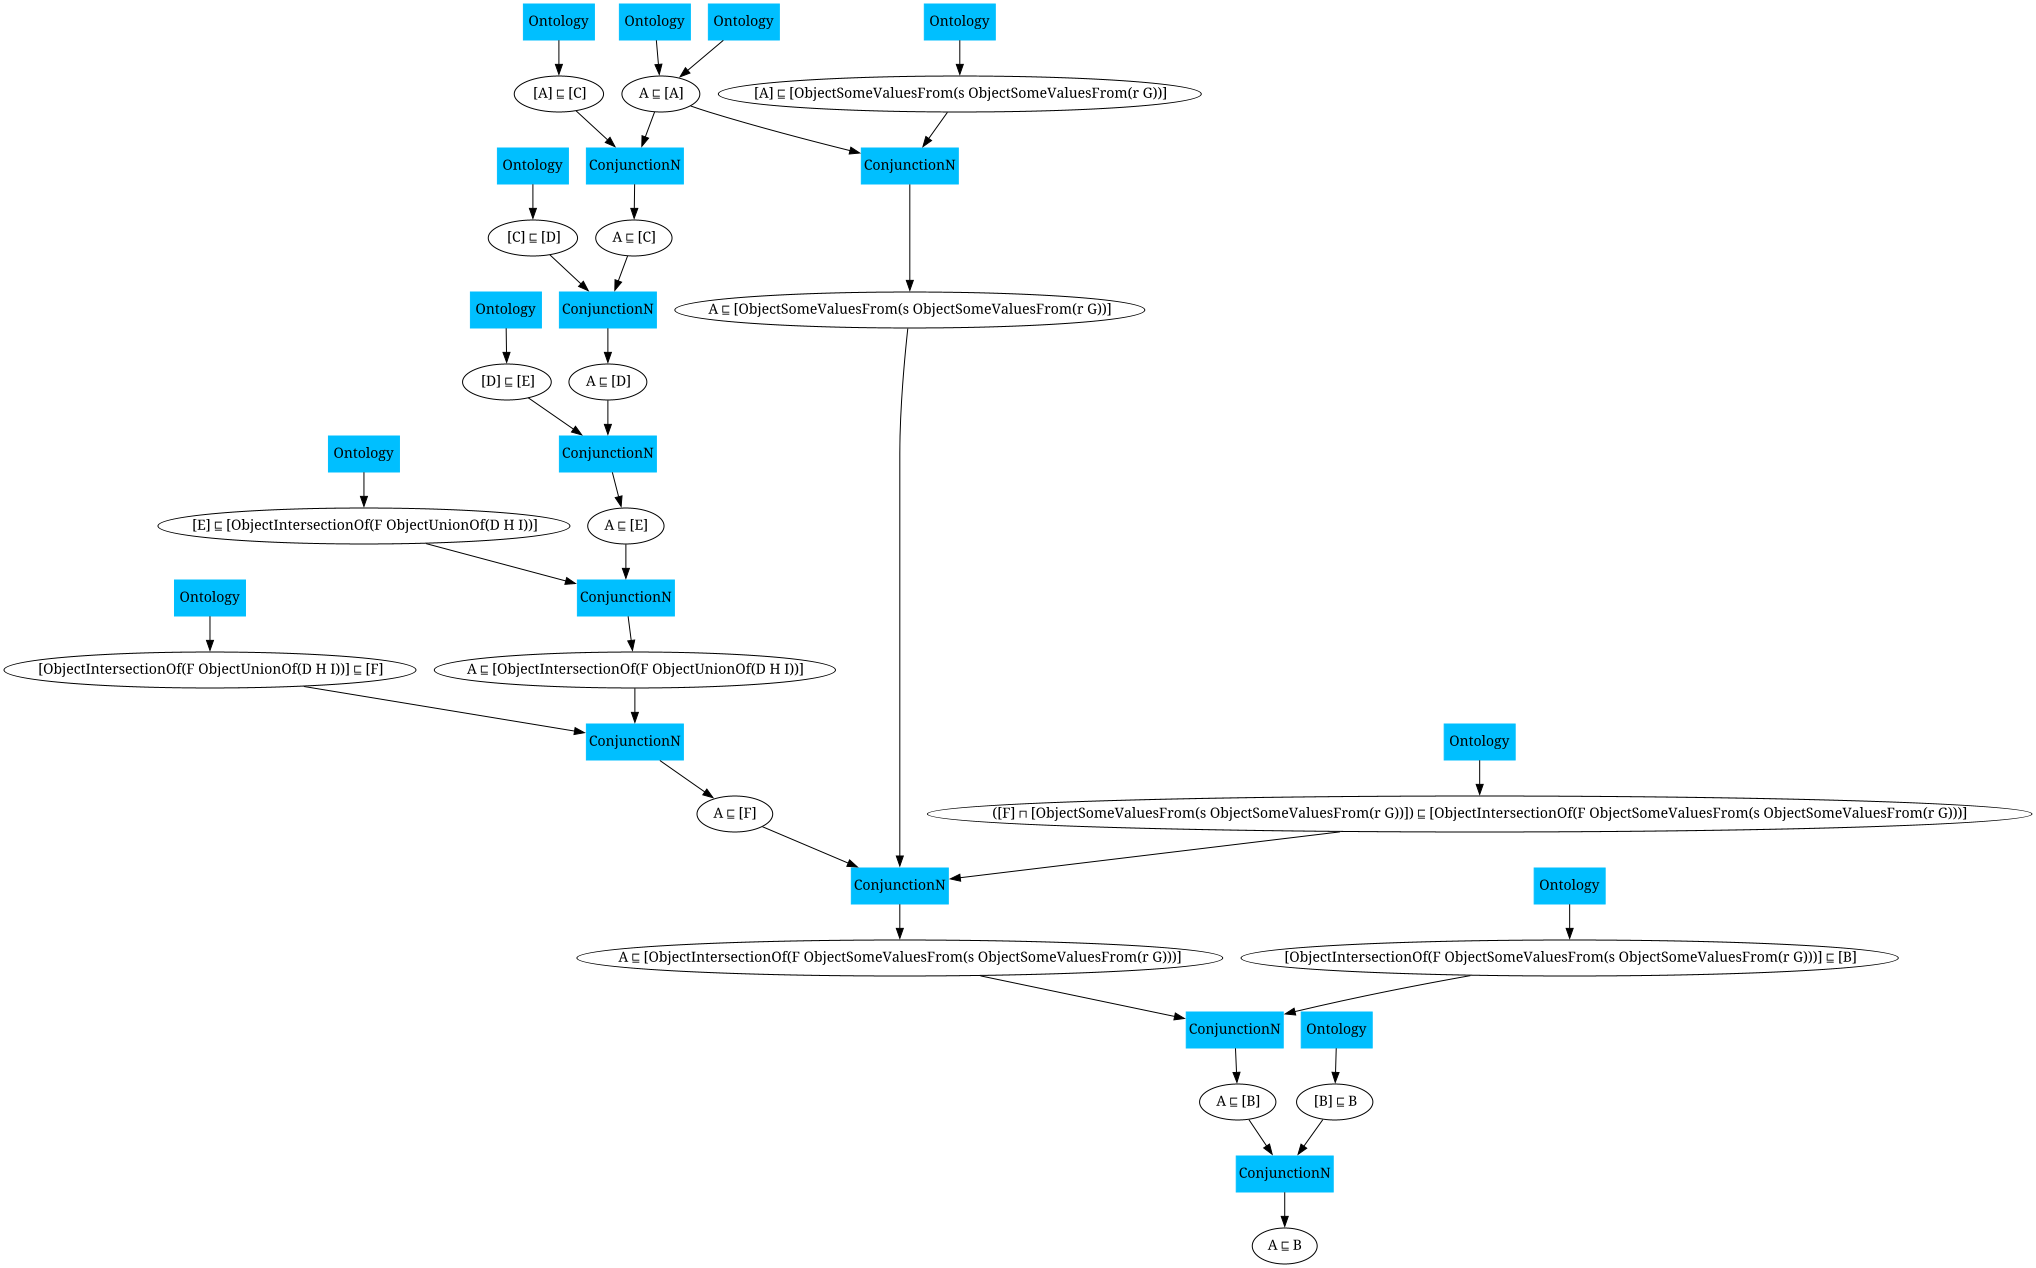
\includegraphics[width=1\textwidth]{pictures/ALCH_task00001.png}
  \caption{ALCH-Reasoner Proof for Task 1}
  \label{fig:t1_Aproof}
\end{figure}


\begin{figure}
  \centering
  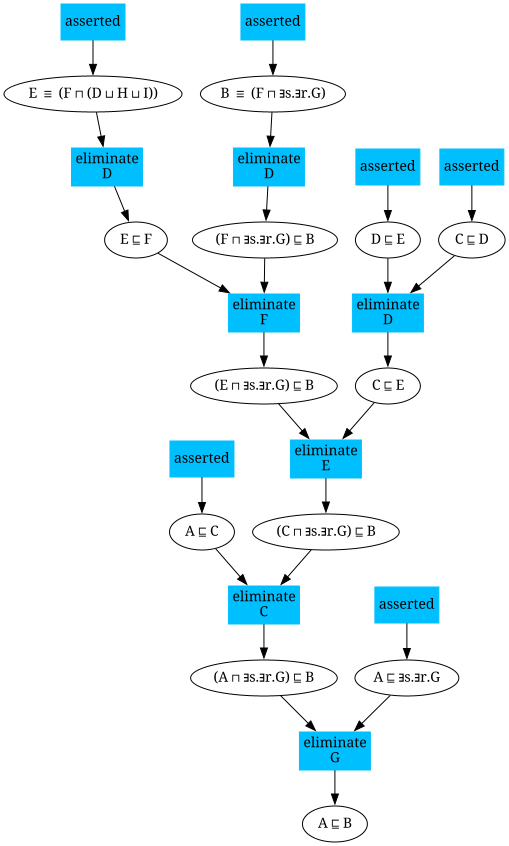
\includegraphics[width=0.6\textwidth]{pictures/Lethe_task00001.png}
  \caption{Lethe Proof for Task 1}
  \label{fig:t1_Lproof}
\end{figure}

When comparing the proofs generated by the ALCH-Reasoner and the Lethe-Reasoner, one can see that the 
proofs differ quite a bit. Also, the number of axioms and rule applications which are used in the proofs
of Lethe are always less than the once of the ALCH-Reasoner, as can be seen in table 
\ref{tab:alch-performance} and \ref{tab:lethe-performance}. 

I see 2 reasons for this. The first reason is that the Lethe-Reasoner uses a different
set of rules than the ALCH-Reasoner.
While for example the ALCH-Reasoner uses only the $\mathbf{R^{n}_{\sqcap}}$ rule
on a normalized task 1 ontology, the Lethe-Reasoner uses quite a few different types of elimination rules.
Also, the interaction between the rules $\mathbf{R^{-}_A}$,$\mathbf{R^{-}_{\exists}}$, $\mathbf{R^\bot_{\exists}}$,
as seen in figure \ref{fig:alch_3}, is quite unintuitive and also blows up the proof. This behavior 
becomes very clear when comparing it to figure \ref{fig:lethe_3}

The second reason is that the structural transformation introduces new concept names for the same concept.
For example for the very simple ontology $ \mathcal{O} = \{ A \sqsubseteq B,  B  \sqsubseteq C \}$ and the GCI $\alpha = A \sqsubseteq C$
one first gets the normalized ontology 
$ \st(\mathcal{O'}) = \{ 
  [A] \sqsubseteq [B], A \sqsubseteq [A], [B] \sqsubseteq B,
  [B] \sqsubseteq [C], B \sqsubseteq [B], [C] \sqsubseteq C \}
$
the proof in \ref{fig:simple_proof} of the GCI $\alpha$ there exist $A$ and $[A]$ which reference to the same concept.
This results in the proof being unnecessarily long and little less readable, since 
we always need an additional step to switch from $A$ to $[A]$ using the $\mathbf{R^{n}_{\sqcap}}$ rule.
Note that this only introduces one more step in the proof and could be prevented by querying for the $[A] \sqsubseteq [B]$
instead.
But the structural transformation introduces also unnecessary in order to unfold the structural transformed
concepts into there semantic valuable representation. For example $A \sqsubseteq [B \sqcap C]$
must first be transformed into $A \sqsubseteq [B] \sqcap [C]$ using the $\mathbf{R^{n}_{\sqcap}}$ rule
before it can interact with axioms like $[B] \sqcap [C] \sqsubseteq [B]$.
This behavior can also be found in figure \ref{fig:unfold}. On could also think about removing such steps
after the reasoning in order to improve the readability of proofs.


%However, just normalizing both sides of the query GCI does not work in the general case since normalization could cause
%the query GCI to be be 


 

\begin{figure}
  \centering
  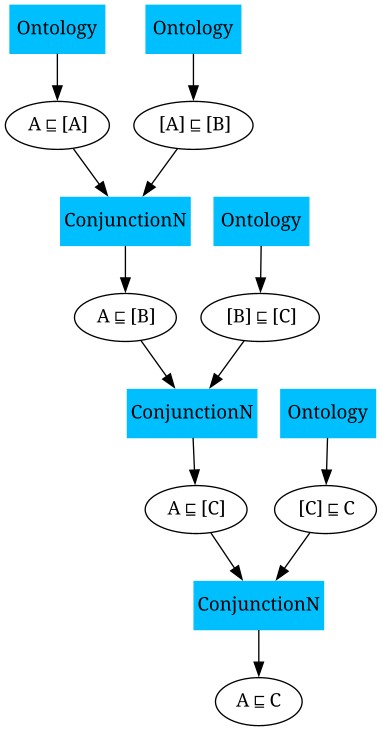
\includegraphics[width=0.4\textwidth]{pictures/longerProofExample2_normalized.png}
  \caption{ALCH simple proof}
  \label{fig:simple_proof}
\end{figure}


\begin{figure}
  \centering
  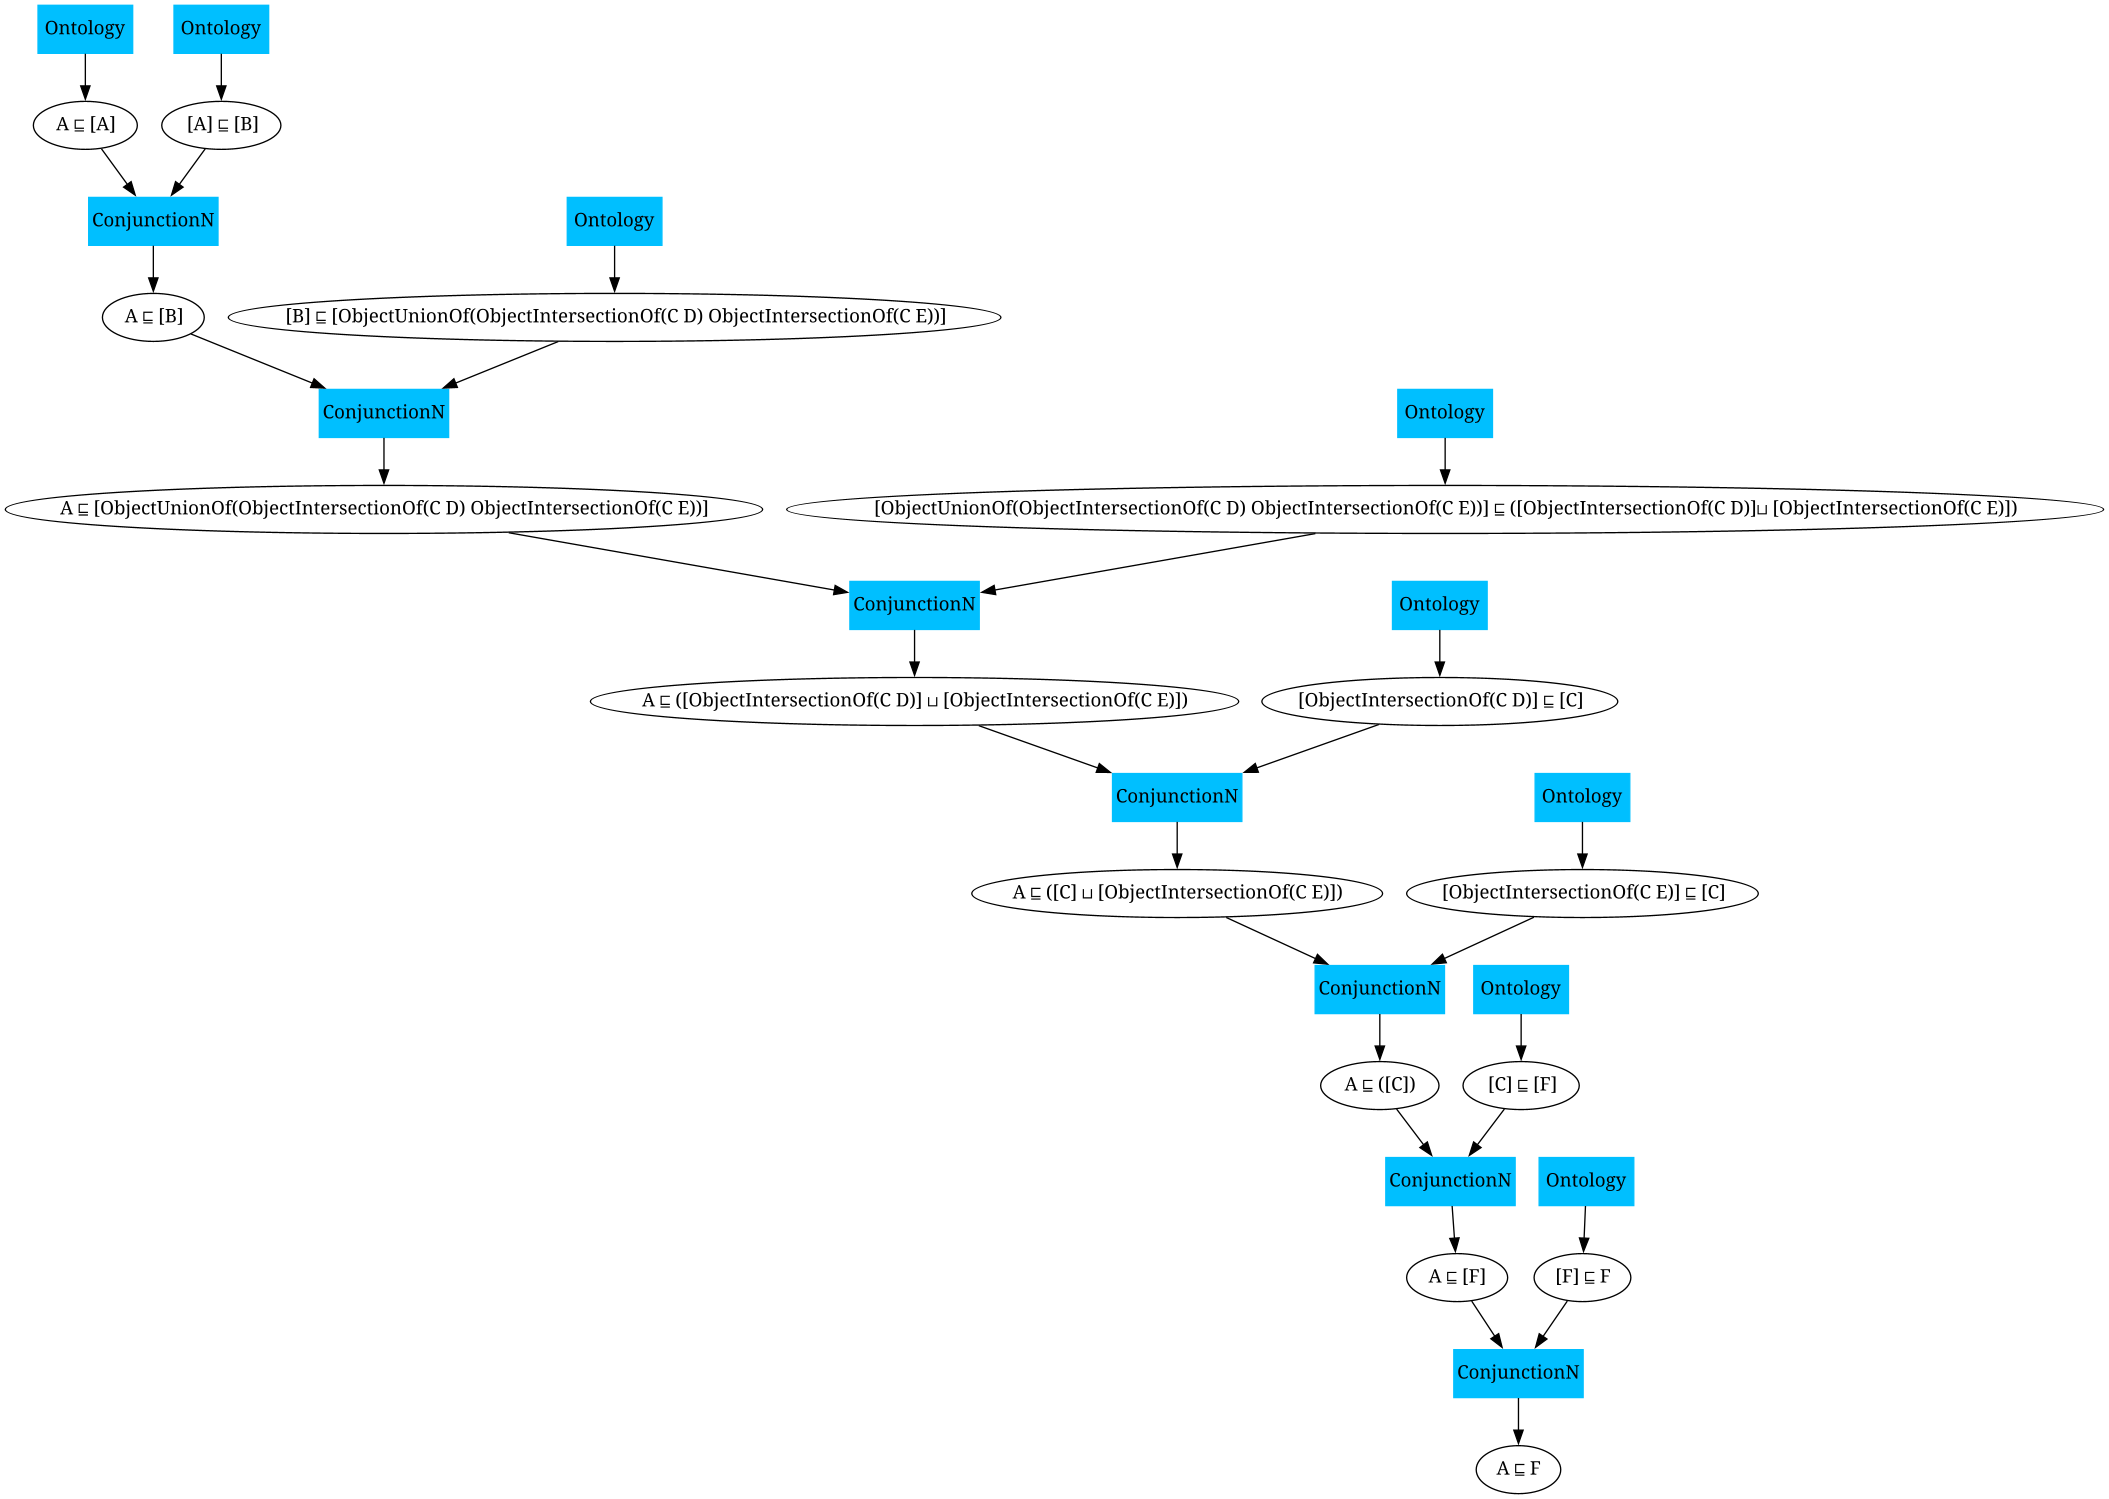
\includegraphics[width=0.8\textwidth]{pictures/ALCH_task00000.png}
  \caption{ALCH unfolding example}
  \label{fig:unfold}
\end{figure}



\begin{figure}
  \centering
  
\includegraphics[width=1\textwidth]{pictures/ALCH_task00003.png}
  \caption{ALCH-Reasoner task 3}
  \label{fig:alch_3}
\end{figure}

\begin{figure}
  \centering
  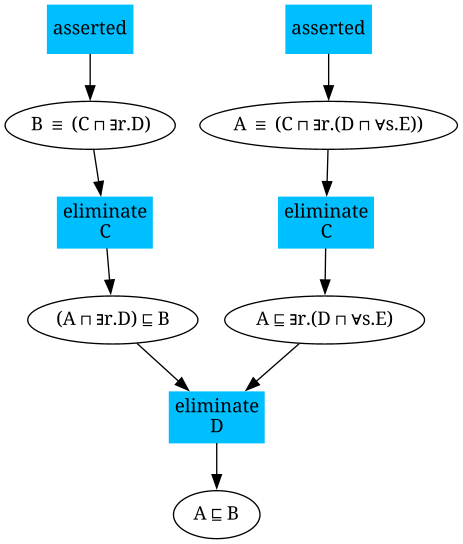
\includegraphics[width=0.5\textwidth]{pictures/Lehte_task00003.png}
  \caption{Lethe task 3}
  \label{fig:lethe_3}
\end{figure}

\subsection{Proofs Time Performance Comparison}
It is interesting to see that in most cases the ALCH-Reasoner is actually around 10 times faster.
When taking a look at task 3 one can see that the rule $\mathbf{R^{-}_{\exists}}$ is used quite often.
I analyzed the behavior of the ALCH-Reasoner and found out that the rule $\mathbf{R^{-}_{\exists}}$ is actually 
applied way more time than any other rule. This is due to the fact that the ALCH-Reasoner does not prune the search
and therefore has to check every option again and again. This behavior is also the case for the rule $\mathbf{R^{n}_{\sqcap}}$ which
produces a lot of combinations in case there is a deep disjunction on the right and side of a concept.
 I also checked this behavior when trying to handle task 13 which contains the axiom
 $A \equiv ((C \sqcap D) \sqcup (C \sqcap E) \sqcup (D \sqcap E) \sqcup (F \sqcap E) \sqcup (C \sqcap F) \sqcup (D \sqcap F))$.
 Unfortunately, this task is too big for the ALCH-Reasoner to handle.


\section{Conclusion}
In conclusion is the ALCH-Reasoner quite fast in most cases and also produces in most cases
quite readable proofs. The ALCH-Reasoner even outperforms Lethe on small, examples which do not
contain big conjunctions or disjunctions nor very complex existential restrictions.
Although there are some things which could be improved.
First one could investigate how to efficiently remove unnecessary reasoning steps.
And secondly there could be way more pruning when searching for axioms of specific forms to improve the performance.
If someone wants to tackle these problems the code and also datasets can be found under \footnote{https://github.com/StBreuer/ALCH-Reasoner.git}
A major flaw probably can not be improved upon is the unintuitive behavior between the 
rules $\mathbf{R^{-}_A}$,$\mathbf{R^{-}_{\exists}}$, $\mathbf{R^\bot_{\exists}}$.
All in all is my implementation is quite fast and also quite readable.

\printbibliography
\end{document} 
